\begin{figure*}
\begin{minipage}{0.25\textwidth}

\begin{subfigure}[b]{\linewidth}
\centering
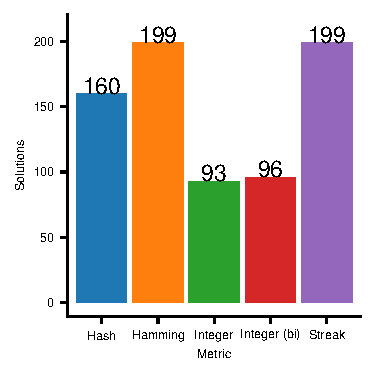
\includegraphics[width=\linewidth]{img/gp_results/panel-cst-sols.pdf}%
\caption{
changing-singal task
}
\label{fig:cst-sols}
\end{subfigure}

\begin{subfigure}[b]{\linewidth}
\centering
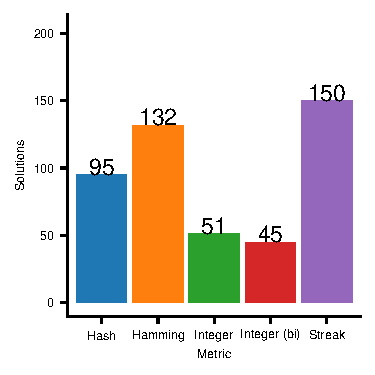
\includegraphics[width=\textwidth]{img/gp_results/panel-dst-sols.pdf}%
\caption{
directional-signal task
}
\label{fig:dst-sols}
\end{subfigure}
\begin{subfigure}[b]{\linewidth}
\centering
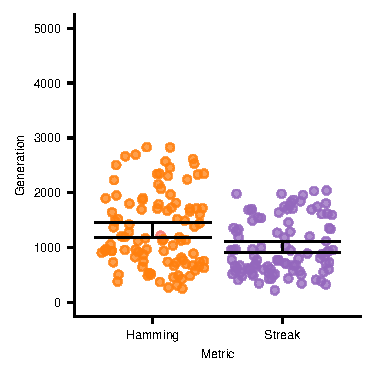
\includegraphics[width=\textwidth]{img/gp_results/panel-dst-times.pdf}%
\caption{
directional-signal task
}
\label{fig:dst-times}
\end{subfigure}

\label{fig:gp_results}

\end{minipage}%
\begin{minipage}{0.75\textwidth}

\begin{subfigure}[b]{\linewidth}
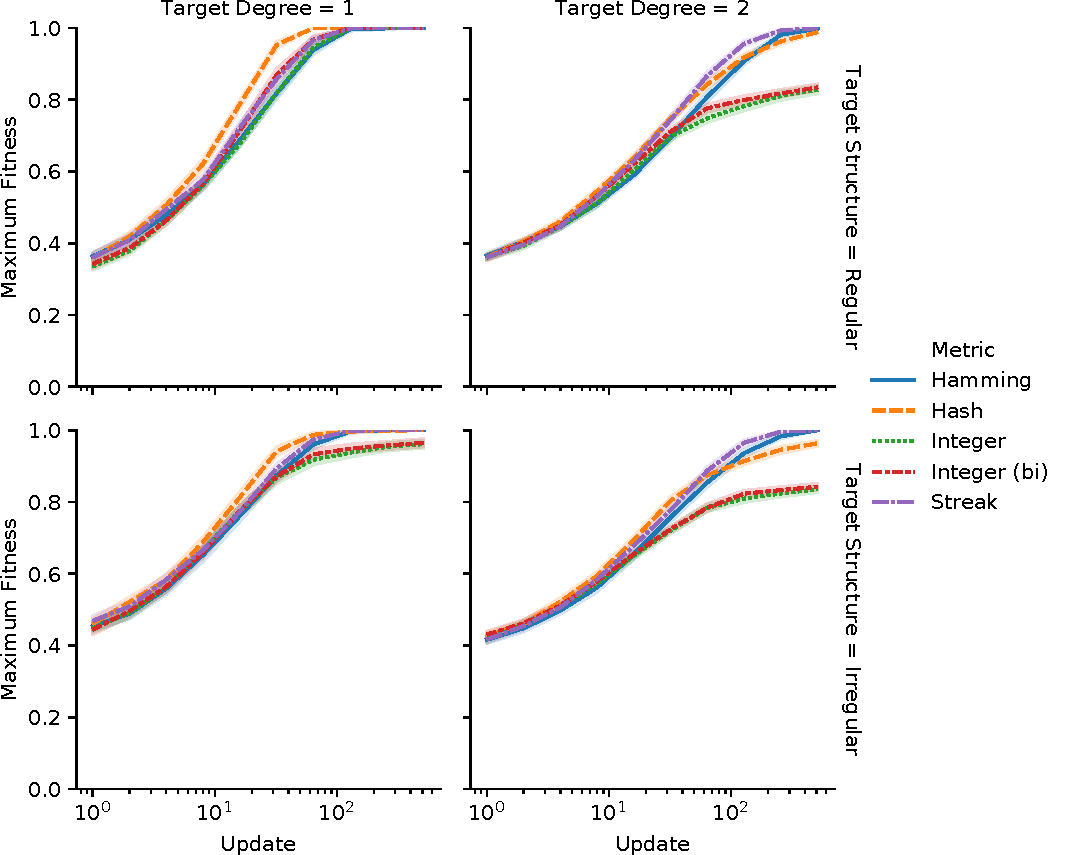
\includegraphics[width=\linewidth]{target_evolve/viz=max-fitness-line+_data_hathash_hash=673d309ab90e91d1+_script_fullcat_hash=fe3ddc711c5abfad+ext=}
%TODO make this a bar graph
\caption{
graph-matching task
}
\label{fig:evolve_bests}
\end{subfigure}

\caption{
Evolutionary analyses of tag-matching metrics.
All show each metrics' best-performing mutation rate.
Figures \ref{fig:cst-sols} and \ref{fig:dst-sols} show the numbers of replicates that produced a complete task solution to the changing-signal and directional-signal task respectively.
Figure \ref{fig:dst-times} show the number of generations elapsed for the first 100 replicates to produce a complete solution to the directional-signal task.
Error bars indicate bootstrapped 95\% confidence intervals around the mean generation.
Figure \ref{fig:evolve_bests} shows maximum fitness by update over replicate runs on the graph-matching task.
Shaded areas represent 95\% confidence intervals.
}
\end{minipage}
\label{fig:evocomposite}
\end{figure*}